%%%%%%%%%%%%%%%%%%%%%%%%%%%%%%%%%%%%%%%%%%%%%%%%%%%%%%%%%%%%%%%%%%%%%%%%%
%  Zawartość: Główny plik szablonu pracy dyplomowej (magisterskiej/inżynierskiej).
%  Opracował: Tomasz Kubik <tomasz.kubik@pwr.edu.pl>
%  Data: kwiecień 2016
%  Wersja: 0.2
%%%%%%%%%%%%%%%%%%%%%%%%%%%%%%%%%%%%%%%%%%%%%%%%%%%%%%%%%%%%%%%%%%%%%%%%%

\documentclass[a4paper,twcolumn,oneside,12pt,extrafontsizes]{memoir}
% W celu przygotowania wydruku do archiwum należy przesłonić komendę powyższą
% dwoma poniższymi komendami:
%\documentclass[a4paper,onecolumn,twoside,10pt]{memoir} 
%\renewcommand{\normalsize}{\fontsize{8pt}{10pt}\selectfont}

%\usepackage[cp1250]{inputenc} % jeśli kodowanie edytowanych plików to cp1250 
\usepackage[utf8]{inputenc} % jeśli kodowanie edytowanych plików to UTF8
\usepackage[T1]{fontenc}
\usepackage[polish]{babel}
%\DisemulatePackage{setspace}
\usepackage{setspace}
\usepackage{tabularx}
\usepackage{color,calc}
%\usepackage{soul} % pakiet z komendami do podkreślania tekstu

\usepackage{ebgaramond} % pakiet z czcionkami garamond, potrzebny tylko do strony tytułowej, musi wystąpić przed pakietem tgtermes

%% Aby uzyskać polskie literki w pdfie (a nie zlepki) korzystamy z pakietu czcionek tgterms. 
%% W pakiecie tym są zdefiniowane klony czcionek Times o kształtach: normalny, pogrubiony, italic, italic pogrubiony.
%% W pakiecie tym brakuje czcionki o kształcie: slanted (podobny do italic). 
%% Jeśli w dokumencie gdzieś zostanie zastosowana czcionka slanted (np. po użyciu komendy \textsl{}), to
%% latex dokona podstawienia na czcionkę standardową i zgłosi to w ostrzeżeniu (warningu).
%% Ponadto tgtermes to czcionka do tekstu. Wszelkie matematyczne wzory będą sformatowane domyślną czcionką do wzorów.
%% Jeśli wzory mają być sformatowane z wykorzystaniem innych czcionek, trzeba to jawnie zadeklarować.

%% Po zainstalowaniu pakietu tgtermes może będzie trzeba zauktualizować informacje 
%% o dostępnych fontach oraz mapy. Można to zrobić z konsoli (jako administrator)
%% initexmf --admin --update-fndb
%% initexmf --admin --mkmaps

\usepackage{tgtermes}   
\renewcommand*\ttdefault{txtt}

% We wcześniejszej wersji szablonu korzystano z innych czcionek. Dla celów historycznych pozostawiono je w komentarzu
%\usepackage{mathptmx} % pakiet będący następcą pakietów times and mathptm, niestety polskie literki są zlepkami
%\usepackage{newtxtext,newtxmath} % pakiety dostarczające Times dla tekstów i wzorów matematycznych,  
%                                  rozwiązuje problemy występujące w mathptmx, ale wymaga zainstalowania
%                                  dodatkowych pakietów oraz uruchomienia updmap (konsola administratora)
%                                  niestety polskie literki są zlepkami
%\usepackage{newtxmath,tgtermes} % można też połączyć czcionki do tekstu i czcionki do wzorów

\usepackage{listings} % pakiet do prezentacji kodu. 
%Wcześniej był problem z polskimi znakami w otoczeniu lstlisting, stąd pozostawiono w komentarzu zastosowane wtedy rozwiązanie: 
\lstset{literate=%-
{ą}{{\k{a}}}1 {ć}{{\'c}}1 {ę}{{\k{e}}}1 {ł}{{\l{}}}1 {ń}{{\'n}}1 {ó}{{\'o}}1 {ś}{{\'s}}1 {ż}{{\.z}}1 {ź}{{\'z}}1 {Ą}{{\k{A}}}1 {Ć}{{\'C}}1 {Ę}{{\k{E}}}1 {Ł}{{\L{}}}1 {Ń}{{\'N}}1 {Ó}{{\'O}}1 {Ś}{{\'S}}1 {Ż}{{\.Z}}1 {Ź}{{\'Z}}1 }%{\ \ }{{\ }}1}

\usepackage[section]{placeins}

% Choć możliwe jest zastosowanie różnych pakietów formatujących tabele, zaleca się tego nie robić.
%\usepackage{longtable}
%\usepackage{ltxtable}
%\usepackage{tabulary}

%%%%%%%%%%%%%%%%%%%%%%%%%%%%%%%%%%%%%%%%%%%%%%%%%%%
%% Ustawienia odpowiedzialne za sposób łamania dokumentu
%% i ułożenie elementów pływających
%%%%%%%%%%%%%%%%%%%%%%%%%%%%%%%%%%%%%%%%%%%%%%%%%%%
%\hyphenpenalty=10000		% nie dziel wyrazów zbyt często
\clubpenalty=10000      %kara za sierotki
\widowpenalty=10000  % nie pozostawiaj wdów
\brokenpenalty=10000		% nie dziel wyrazów między stronami
\exhyphenpenalty=999999		% nie dziel słów z myślnikiem
\righthyphenmin=3			% dziel minimum 3 litery

%\tolerance=4500
%\pretolerance=250
%\hfuzz=1.5pt
%\hbadness=1450

\renewcommand{\topfraction}{0.95}
\renewcommand{\bottomfraction}{0.95}
\renewcommand{\textfraction}{0.05}
\renewcommand{\floatpagefraction}{0.35}

%%%%%%%%%%%%%%%%%%%%%%%%%%%%%%%%%%%%%%%%%%%%%%%%%%%
%%  Ustawienia rozmiarów: tekstu, nagłówka i stopki, marginesów
%%  dla dokumentów klasy memoir 
%%%%%%%%%%%%%%%%%%%%%%%%%%%%%%%%%%%%%%%%%%%%%%%%%%%
\setlength{\headsep}{10pt} 
\setlength{\headheight}{13.6pt} % wartość baselineskip dla czcionki 11pt tj. \small wynosi 13.6pt
\setlength{\footskip}{\headsep+\headheight}
\setlength{\uppermargin}{\headheight+\headsep+1cm}
\setlength{\textheight}{\paperheight-\uppermargin-\footskip-1.5cm}
\setlength{\textwidth}{\paperwidth-5cm}
\setlength{\spinemargin}{2.5cm}
\setlength{\foremargin}{2.5cm}
\setlength{\marginparsep}{2mm}
\setlength{\marginparwidth}{2.3mm}
%\settrimmedsize{297mm}{210mm}{*}
%\settrims{0mm}{0mm}	
\checkandfixthelayout[fixed] % konieczne, aby się dobrze wszystko poustawiało
%%%%%%%%%%%%%%%%%%%%%%%%%%%%%%%%%%%%%%%%%%%%%%%%
%%  Ustawienia odległości linii, wcięć, odstępów
%%%%%%%%%%%%%%%%%%%%%%%%%%%%%%%%%%%%%%%%%%%%%%%%
\linespread{1}
%\linespread{1.241}
\setlength{\parindent}{14.5pt}
\setbeforesecskip{10pt plus 0.5ex}%{-3.5ex \@plus -1ex \@minus -.2ex}
\setaftersecskip{10pt plus 0.5ex}%\onelineskip}
\setbeforesubsecskip{8pt plus 0.5ex}%{-3.5ex \@plus -1ex \@minus -.2ex}
\setaftersubsecskip{8pt plus 0.5ex}%\onelineskip}
\setbeforesubsubsecskip{8pt plus 0.5ex}%{-3.5ex \@plus -1ex \@minus -.2ex}
\setlength\floatsep{6pt plus 2pt minus 2pt} 
\setlength\intextsep{12pt plus 2pt minus 2pt} 
\setlength\textfloatsep{12pt plus 2pt minus 2pt} 

%%%%%%%%%%%%%%%%%%%%%%%%%%%%%%%%%%%%%%%%%%%%%%%%%%%
%%  Pakiety i komendy zastosowane tylko do zamieszczenia informacji o użytych komendach i fontach
%%  Normalnie nie są potrzebne, można je zamarkować podczas redakcji pracy
%%%%%%%%%%%%%%%%%%%%%%%%%%%%%%%%%%%%%%%%%%%%%%%%%%%
\usepackage{memlays}     % extra layout diagrams, zastosowane w szblonie do 'debuggowania', używa pakietu layouts
%\usepackage{layouts}
\usepackage{printlen} % pakiet do wyświetlania wartości zdefiniowanych długości, stosowany do 'debuggowania'
\uselengthunit{pt}
\makeatletter
\newcommand{\showFontSize}{\f@size pt} % makro wypisujące wielkość bieżącej czcionki
\makeatother
% do pokazania ramek można byłoby użyć:
%\usepackage{showframe} 

\usepackage{indentfirst}
\usepackage{textgreek}

%%%%%%%%%%%%%%%%%%%%%%%%%%%%%%%%%%%%%%%%%%%%%%%%%%%
%%  Formatowanie list wyliczeniowych, wypunktowań i własnych otoczeń
%%%%%%%%%%%%%%%%%%%%%%%%%%%%%%%%%%%%%%%%%%%%%%%%%%%

% Domyślnie wypunktowania mają zadeklatorowane znaki, które nie występują w tgtermes
% Aby latex nie podstawiał w ich miejsca znaków z czcionki standardowej można zrobić podstawienie:
%    \DeclareTextCommandDefault{\textbullet}{\ensuremath{\bullet}}
%    \DeclareTextCommandDefault{\textasteriskcentered}{\ensuremath{\ast}}
%    \DeclareTextCommandDefault{\textperiodcentered}{\ensuremath{\cdot}}
% Jednak jeszcze lepszym pomysłem jest zdefiniowanie otoczeń z wykorzystaniem enumitem
\usepackage{enumitem} % pakiet pozwalający zarządzać formatowaniem list wyliczeniowych
\setlist{noitemsep,topsep=4pt,parsep=0pt,partopsep=4pt,leftmargin=*} % zadeklarowane parametry pozwalają uzyskać 'zwartą' postać wypunktowania bądź wyliczenia
\setenumerate{labelindent=0pt,itemindent=0pt,leftmargin=!,label=\arabic*.} % można zmienić \arabic na \alph, jeśli wyliczenia mają być z literkami
\setlistdepth{4} % definiujemy głębokość zagnieżdżenia list wyliczeniowych do 4 poziomów
\setlist[itemize,1]{label=$\bullet$}  % definiujemy, jaki symbol ma być użyty w wyliczeniu na danym poziomie
\setlist[itemize,2]{label=\normalfont\bfseries\textendash}
\setlist[itemize,3]{label=$\ast$}
\setlist[itemize,4]{label=$\cdot$}
\renewlist{itemize}{itemize}{4}

%%%http://tex.stackexchange.com/questions/29322/how-to-make-enumerate-items-align-at-left-margin
%\renewenvironment{enumerate}
%{
%\begin{list}{\arabic{enumi}.}
%{
%\usecounter{enumi}
%%\setlength{\itemindent}{0pt}
%%\setlength{\leftmargin}{1.8em}%{2zw} % 
%%\setlength{\rightmargin}{0zw} %
%%\setlength{\labelsep}{1zw} %
%%\setlength{\labelwidth}{3zw} % 
%\setlength{\topsep}{6pt}%
%\setlength{\partopsep}{0pt}%
%\setlength{\parskip}{0pt}%
%\setlength{\parsep}{0em} % 
%\setlength{\itemsep}{0em} % 
%\setlength{\listparindent}{1zw} % 
%}
%}{
%\end{list}
%}

\makeatletter
\renewenvironment{quote}{
	\begin{list}{}
	{
	\setlength{\leftmargin}{1em}
	\setlength{\topsep}{0pt}%
	\setlength{\partopsep}{0pt}%
	\setlength{\parskip}{0pt}%
	\setlength{\parsep}{0pt}%
	\setlength{\itemsep}{0pt}
	}
	}{
	\end{list}}
\makeatother

%%%%%%%%%%%%%%%%%%%%%%%%%%%%%%%%%%%%%%%%%
%%  Pakiet do generowania indeksu (ważne, aby wstawić przed hyperref)
%%%%%%%%%%%%%%%%%%%%%%%%%%%%%%%%%%%%%%%%%
\DisemulatePackage{imakeidx}
\usepackage[makeindex,noautomatic]{imakeidx} % tutaj mówimy, żeby indeks nie generował się automatycznie, 

%\usepackage[noautomatic]{imakeidx} 
\makeindex

\makeatletter
%%%\renewenvironment{theindex}
							 %%%{\vskip 10pt\@makeschapterhead{\indexname}\vskip -3pt%
								%%%\@mkboth{\MakeUppercase\indexname}%
												%%%{\MakeUppercase\indexname}%
								%%%\vspace{-3.2mm}\parindent\z@%
								%%%\renewcommand\subitem{\par\hangindent 16\p@ \hspace*{0\p@}}%%
								%%%\phantomsection%
								%%%\begin{multicols}{2}
								%%%%\thispagestyle{plain}
								%%%\parindent\z@                
								%%%%\parskip\z@ \@plus .3\p@\relax
								%%%\let\item\@idxitem}
							 %%%{\end{multicols}\clearpage}
%%%
\makeatother


\usepackage{ifpdf}
%\newif\ifpdf \ifx\pdfoutput\undefined
%\pdffalse % we are not running PDFLaTeX
%\else
%\pdfoutput=1 % we are running PDFLaTeX
%\pdftrue \fi
\ifpdf
 \usepackage[pdftex,bookmarks,breaklinks,unicode]{hyperref}
 \usepackage[pdftex]{graphicx}
 \DeclareGraphicsExtensions{.pdf,.jpg,.mps,.png}
\pdfcompresslevel=9
\pdfoutput=1
\makeatletter
\AtBeginDocument{
  \hypersetup{
	pdfinfo={
    Title = {\@title},
    Author = {\@author},
    Subject={},
    Keywords={słowa kluczowe},
  }}
}
\makeatother
\else
\usepackage{graphicx}
\DeclareGraphicsExtensions{.eps,.ps,.jpg,.mps,.png}
\fi
\sloppy


%\graphicspath{{rys01/}{rys02/}}


%%%%%%%%%%%%%%%%%%%%%%%%%%%%%%%%%%%%%%%%%
% Metadane dla pdfa


%\ifpdf
%\pdfinfo{
   %/Author (Nicola Talbot)
   %/Title  (Creating a PDF document using PDFLaTeX)
   %/CreationDate (D:20040502195600)
   %/ModDate (D:\pdfdate)
   %/Subject (PDFLaTeX)
   %/Keywords (PDF;LaTeX)
%}
%\fi

% Deklaracja głębokościu numeracji
\setcounter{secnumdepth}{2}
\setcounter{tocdepth}{2}
\setsecnumdepth{subsection} % activating subsubsec numbering in doc


% Kropki po numerach sekcji
\makeatletter
\def\@seccntformat#1{\csname the#1\endcsname.\quad}
\def\numberline#1{\hb@xt@\@tempdima{#1\if&#1&\else.\fi\hfil}}
\makeatother

\renewcommand{\chapternumberline}[1]{#1.\quad}
\renewcommand{\cftchapterdotsep}{\cftdotsep}

%\definecolor{niceblue}{rgb}{.168,.234,.671}

% Czcionka do podpisów tabel i rysunków
\captionnamefont{\small}
\captiontitlefont{\small}
% makro pozwalające zmienić sposób wypisywania rozdziału
%\def\printchaptertitle##1{\fonttitle \space \thechapter.\space ##1} 

%\usepackage{ltcaption}
% The ltcaption package supports \CaptionLabelFont & \CaptionTextFont introduced by the NTG document classes
%\renewcommand\CaptionLabelFont{\small}
%\renewcommand\CaptionTextFont{\small}

% Przedefiniowanie etykiet w podpisach tabel i rysunków
%\AtBeginDocument{% 
        \addto\captionspolish{% 
        \renewcommand{\tablename}{Tab.}% 
}%} 

%\AtBeginDocument{% 
%        \addto\captionspolish{% 
%        \renewcommand{\chaptername}{Rozdział}% 
%}} 

%\AtBeginDocument{% 
        \addto\captionspolish{% 
        \renewcommand{\figurename}{Rys.}% 
}%}


%\AtBeginDocument{% 
        \addto\captionspolish{% 
        \renewcommand{\bibname}{Literatura}% 
}%}


%%%%%%%%%%%%%%%%%%%%%%%%%%%%%%%%%%%%%%%%%%%%%%%%%%%%%%%%%%%%%%%%%%                  
%% Definicje stopek i nagłówków
%%%%%%%%%%%%%%%%%%%%%%%%%%%%%%%%%%%%%%%%%%%%%%%%%%%%%%%%%%%%%%%%%%                  
\addtopsmarks{headings}{%
\nouppercaseheads % added at the beginning
}{%
\createmark{chapter}{both}{shownumber}{}{. \space}
%\createmark{chapter}{left}{shownumber}{}{. \space}
\createmark{section}{right}{shownumber}{}{. \space}
}%use the new settings

\makeatletter
\copypagestyle{outer}{headings}
\makeoddhead{outer}{}{}{\small\itshape\rightmark}
\makeevenhead{outer}{\small\itshape\leftmark}{}{}
\makeoddfoot{outer}{\small\@author:~\@titleShort}{}{\small\thepage}
\makeevenfoot{outer}{\small\thepage}{}{\small\@author:~\@title}
\makeheadrule{outer}{\linewidth}{\normalrulethickness}
\makefootrule{outer}{\linewidth}{\normalrulethickness}{2pt}
\makeatother

% fix plain
\copypagestyle{plain}{headings} % overwrite plain with outer
\makeoddhead{plain}{}{}{} % remove right header
\makeevenhead{plain}{}{}{} % remove left header
\makeevenfoot{plain}{}{}{}
\makeoddfoot{plain}{}{}{}

\copypagestyle{empty}{headings} % overwrite plain with outer
\makeoddhead{empty}{}{}{} % remove right header
\makeevenhead{empty}{}{}{} % remove left header
\makeevenfoot{empty}{}{}{}
\makeoddfoot{empty}{}{}{}


%%%%%%%%%%%%%%%%%%%%%%%%%%%%%%%%%%%%%%%
%% Definicja strony tytułowej 
%%%%%%%%%%%%%%%%%%%%%%%%%%%%%%%%%%%%%%%
\makeatletter
%Uczelnia
\newcommand\uczelnia[1]{\renewcommand\@uczelnia{#1}}
\newcommand\@uczelnia{}
%Wydział
\newcommand\wydzial[1]{\renewcommand\@wydzial{#1}}
\newcommand\@wydzial{}
%Kierunek
\newcommand\kierunek[1]{\renewcommand\@kierunek{#1}}
\newcommand\@kierunek{}
%Specjalność
\newcommand\specjalnosc[1]{\renewcommand\@specjalnosc{#1}}
\newcommand\@specjalnosc{}
%Tytuł po angielsku
\newcommand\titleEN[1]{\renewcommand\@titleEN{#1}}
\newcommand\@titleEN{}
%Tytuł krótki
\newcommand\titleShort[1]{\renewcommand\@titleShort{#1}}
\newcommand\@titleShort{}
%Promotor
\newcommand\promotor[1]{\renewcommand\@promotor{#1}}
\newcommand\@promotor{}

%\usepackage[absolute]{textpos} % zamarkowano, bo ostatecznie wykorzystano otoczenie picture

\def\maketitle{%
  \pagestyle{empty}%
%%\garamond 
	\fontfamily{\ebgaramond@family}\selectfont % na stronie tytułowej czcionka garamond
%%%%%%%%%%%%%%%%%%%%%%%%%%%%%%%%%%%%%	
%% Poniżej, w otoczniu picture, wstawiono tytuł i autora. 
%% Tytuł (z autorem) musi znaleźć się w obszarze 
%% odpowiadającym okienku 110mmx75mm, którego lewy górny róg 
%% jest w położeniu 77mm od lewej i 111mm od górnej  krawędzi strony 
%% (tak wynika z wycięcia na okładce). 
%% Poniższy kod musi być użyty dokładnie w miejscu gdzie jest.
%% Jeśli tytuł nie mieści się w okienku, to należy tak pozmieniać 
%% parametry użytych komend, aby ten przydługi tytuł jednak 
%% upakować go do okienka.
%%
%% Sama okładka (kolorowa strona z wycięciem, do pobrania z dydaktyki) 
%% powinna być przycięta o 3mm od każdej z krawędzi.
%% Te 3mm pewnie zostawiono na ewentualne spady czy też specjalną oprawę.
%%%%%%%%%%%%%%%%%%%%%%%%%%%%%%%%%%%%%	
\newlength{\tmpfboxrule}
\setlength{\tmpfboxrule}{\fboxrule}
\setlength{\fboxsep}{2mm}
\setlength{\fboxrule}{0mm} 
%\setlength{\fboxrule}{0.1mm} %% jeśli chcemy zobaczyć ramkę
\setlength{\unitlength}{1mm}
\begin{picture}(0,0)
\put(26,-124){\fbox{
\parbox[c][71mm][c]{104mm}{\centering%\lineskip=34pt 
\fontsize{16pt}{18pt}\selectfont \@title\\[5mm]
\fontsize{16pt}{18pt}\selectfont \@titleEN\\[20mm]
\fontsize{16pt}{18pt}\selectfont AUTOR:\\[2mm]
\fontsize{14pt}{16pt}\selectfont \@author}
}
}
\end{picture}
\setlength{\fboxrule}{\tmpfboxrule} 
%%%%%%%%%%%%%%%%%%%%%%%%%%%%%%%%%%%%%
%% Reszta strony z nazwą uczelni, wydziału, kierunkiem, specjalnością
%% promotorem, oceną pracy, miastem i rokiem
	{\centering%\vspace{-1cm}
		{\fontsize{22pt}{24pt}\selectfont \@uczelnia}\\[0.4cm]
		{\fontsize{22pt}{24pt}\selectfont \@wydzial}\\[0.5cm]
		  \hrule %\vspace*{0.7cm}
	}
{\flushleft\fontsize{14pt}{16pt}\selectfont%
\begin{tabular}{ll}
KIERUNEK: & \@kierunek\\
SPECJALNOŚĆ: & \@specjalnosc\\
\end{tabular}\\[1.3cm]
}
{\centering
{\fontsize{32pt}{36pt}\selectfont PRACA DYPLOMOWA}\\[0.5cm]
{\fontsize{32pt}{36pt}\selectfont INŻYNIERSKA}\\[2.5cm]
}
\vfill
\begin{tabularx}{\linewidth}{p{6cm}l}
		&{\fontsize{16pt}{18pt}\selectfont PROWADZĄCY PRACĘ:}\\[2mm] %UWAGA: tutaj jest miejsce na nazwisko promotora pracy
		&{\fontsize{14pt}{16pt}\selectfont \@promotor}\\[10mm]
		&{\fontsize{16pt}{18pt}\selectfont OCENA PRACY:}\\[20mm]
	\end{tabularx}
\vspace{2cm}
\hrule\vspace*{0.3cm}
{\centering
{\fontsize{16pt}{18pt}\selectfont \@date}\\[0cm]
}
%\ungaramond
\normalfont
 \cleardoublepage
}
\makeatother
%%%%%%%%%%%%%%%%%%%%%%%%%%%%%%%%%%%%%%%%%

%\AtBeginDocument{\addtocontents{toc}{\protect\thispagestyle{empty}}}




%%%%%%%%%%%%%%%%%%%%%%%%%%%%%%%%%%%%%%%%%
%%  Metadane dokumentu 
%%%%%%%%%%%%%%%%%%%%%%%%%%%%%%%%%%%%%%%%%
\title{Aplikacja do obliczania i wyświetlania informacji o aktualnym stanie pojazdu oparta o platformę Arduino}
\titleShort{Aplikacja do obliczania i wyświetlania informacji o aktualnym stanie...}
\titleEN{Application for calculating and displaying data about vehicle's status based on the Arduino platform}
\author{Szymon Sakowicz}
\uczelnia{POLITECHNIKA WROCŁAWSKA}
\wydzial{WYDZIAŁ ELEKTRONIKI}
\kierunek{TELEINFORMATYKA}
\specjalnosc{PROJEKTOWANIE SIECI TELEINFORMATYCZNYCH}
\promotor{dr inż. Arkadiusz Grzybowski W4/K2}
\date{WROCŁAW, 2019}

% Ustawienie odstępu od góry w nienumerowanych rozdziałach oraz wykazach:
% Spis treści, Spis tabel, Spis rysunków, Indeks rzeczowy

%\newlength{\linespace}
%\setlength{\linespace}{-\beforechapskip-\topskip+\headheight+\topsep}
%\makechapterstyle{noNumbered}{%
%\renewcommand\chapterheadstart{\vspace*{\linespace}}
%}

%% powyższa komenda załatwia to, co robią komendy poniższe dla spisów
%\renewcommand*{\tocheadstart}{\vspace*{\linespace}}
%\renewcommand*{\lotheadstart}{\vspace*{\linespace}}
%\renewcommand*{\lofheadstart}{\vspace*{\linespace}}

%%%%%%%%%%%%%%%%%%%%%%%%%%%%%%%%%%%%%%%%%
%                  Początek dokumentu 
%%%%%%%%%%%%%%%%%%%%%%%%%%%%%%%%%%%%%%%%%
%\includeonly{skroty,rozdzial01} % jeśli chcemy kompilować tylko fragmenty, to można tu je wpisać

\begin{document}
% Tutaj można przełączyć odstęp między liniami
%\SingleSpacing
%\OnehalfSpacing
%\DoubleSpacing

%\settypeoutlayoutunit{cm} % do debugowania
%\typeoutstandardlayout    % wypisuje na stdout informacje o ustawieniach
\maketitle

\newpage


\chapterstyle{noNumbered}
\pagestyle{outer}
\mbox{}\pdfbookmark[0]{Spis treści}{spisTresci.1}
\tableofcontents* 

% \newpage
% \mbox{}\pdfbookmark[0]{Spis rysunków}{spisRysunkow.1}
% %\addcontentsline{toc}{chapter}{Spis rysunków}
% \listoffigures*
% \begin{flushleft}

% \end{flushleft}
% %{%
%\let\oldnumberline\numberline%
%\renewcommand{\numberline}{\figurename~\oldnumberline}%
%\listoffigures%
%}


% \newpage
% \mbox{}\pdfbookmark[0]{Spis tabel}{spisTabel.1}
% %\addcontentsline{toc}{chapter}{Spis tabel}
% \listoftables*

% \chapter*{Skróty}\mbox{}\pdfbookmark[0]{Skróty}{skroty.1}
\label{sec:skroty}
\noindent
\begin{description}
  \item [VSS] (ang.\ \emph{Vehicle Speed Sensor})
  \item [ECU] (ang.\ \emph{Engine Control Unit})
  \item [TPS] (ang.\ \emph{Throttle Postion Sensor})
  \item [INJ] (ang.\ \emph{Fuel Injector})
\end{description}
 %skróty można sobie pominąć
\chapterstyle{default}
\chapter{Wstęp}
\section{Motywacja}
Starsze samochody nie posiadają wskaźników czy komputerów pokładowych, które informują na temat poziomu spalania pojazdu. Wiele z nich nie posiada również złącz diagnostycznych, które umożliwiają wyprowadzenie takich danych na zewnątrz. Posiadając podstawową wiedzę na temat działania silnika spalinowego oraz posługując się obliczeniami matematycznymi można wyprowadzić te informacje dla użytkownika samochodu. Z pomocą przychodzą mikrokontrolery.
\section{Cel}
Celem pracy jest stworzenie oraz implementacja urządzenia do wyświetlania aktualnego oraz średniego spalania pojazdu. Projekt ma wykorzystywać mikrokontroler Arduino oparty na architekturze AVR.
\\Celem pobocznym jest wykonanie przyjaznego interfejsu umożliwiającego przekazanie tych informacji użytkownikowi pojazdu. Dodatkowo system powinien wyświetlać informacje na temat prędkości, aktualnej temperatury, aktualnego poziomu napięcia w układzie pojazdu, aktualnego położenia pedału gazu oraz zapisywać archiwalne dane dotyczące spalania w pamięci nieulotnej.
\section{Zakres i układ pracy}
W rozdziale drugim opisana jest ogólna zasadza działania oraz założenia projektu. W tym dziale określono teoretycznie i matematycznie w jaki sposób obliczane są potrzebne dane. W trzecim rozdziale opisana jest fizyczna implementacja projektu: w jaki sposób podłączone są przewody, w jaki sposób działają moduły oraz w jakie układy są połączone. Rozdział czwarty obejmuje programowanie modułu, tj. zastosowanie matematycznych obliczeń w kodzie programu oraz konfigurowanie i inicjalizacja modułu. W rozdziale piątym opisano programowanie interfejsu oraz działanie programu, na które ma wpływ użytkownik. Ostatnim rozdziałem jest podsumowanie, w którym opisano również możliwości rozbudowy.
\chapter{Założenia i zasada działania}
\section{Założenia}
\subsection{Pojazd}
Projekt będzie tworzony przykładzie pojazdu Honda Civic VI z silnikiem D14A8 z roku 1998.

\section{Zasada działania}
\subsection{Potrzebne dane}
Do odczytania informacji potrzebnych do obliczenia aktualnego spalania potrzebujemy dwóch głównych informacji:
\begin{itemize}
\item{aktualnej prędkości pojazdu}
\item{ilości wstrzykiwanego paliwa na jednostkę czasu}
\end{itemize}

\subsection{Obliczanie aktualnej prędkości pojazdu}
Do tego celu potrzebny będzie sygnał, który wysyła VSS (Vehicle Speed Sensor) - jest to urządzenie, z którego korzysta wskaźnik prędkości na desce rozdzielczej. W ogólnym założeniu działa on tak, iż wysyła określoną ilość impulsów co określony dystans. W przypadku pojazdu, na którym budowany jest projekt jest to \textbf{4000 impulsów} co \textbf{jedną milę}.\\
\\Jeżeli prędkość będziemy odświeżać co sekundę, oraz po odświeżeniu będziemy resetować ilość impulsów VSS to prędkość obliczymy z wzoru (zobacz równanie (\ref{eq:speed})).

\begin{equation}\label{eq:speed}
V[km/h] = \frac{S[km]}{I} 3600 i
\end{equation}
gdzie:
\begin{description}
\item[S] długość jednostki dystansu, w przeliczeniu na kilometry, w której VSS wysyła sygnał
\item[I] to stała liczba impulsów VSS, co którą pojazd pokonuje określony dystans
\item[i] to liczba impulsów w tej sekundzie
\end{description}
W przypadku tego pojazdu wzór przedstawia się następująco (zobacz równanie (\ref{eq:speed2})).
\begin{equation}\label{eq:speed2}
V[km/h] = \frac{1.609344[km]}{4000} 3600i
\end{equation}

\subsection{Obliczanie spalania}
Koncepcja obliczania spalania polega na mierzeniu czasu otwarcia wtrysku, czyli czasu, w którym paliwo jest wstrzykiwane do komory spalania silnika. Jeśli znamy stałą wtryskiwacza, czyli parametr mówiący jaka ilość paliwa jest wtryskiwana w danym okresie czasu, możemy obliczyć aktualne spalanie samochodu.\\
Pojazd, na którym oparta jest ta praca posiada wtryski 190cc, co oznacza, że wtryskują one \textbf{190 ml paliwa na minutę}.

\subsubsection{Obliczanie spalania na godzinę}
W tym wypadku również, jak w przypadku prędkości, co jedną sekundę sprawdzamy, przez jaki czas wtrysk wstrzykiwał paliwo. Mając już tę informację spalanie na godzinę wyliczamy ze wzoru(\ref{eq:consumptionPerHour}))

\begin{equation}\label{eq:consumptionPerHour}
C_{h}[L/h] = N\frac{I[ml]}{60}\frac{i[\mu s]}{1000000}\frac{3600}{1000}
\end{equation}
gdzie:
\begin{description}
\item[N] to ilość wtrysków w silniku
\item[I] to stała wtrysku
\item[i] to czas otwarcia wtrysku w danej sekundzie
\end{description}
Należałoby tutaj zaznaczyć, iż w tym projekcie pobierana jest informacja tylko z jednego wtrysku. Każdy wtrysk wstrzykuje za każdym razem tyle samo paliwa, więc ewentualny błąd przybliżenia do N wtrysków jest pomijalny.
\subsubsection{Obliczanie aktualnego spalania na 100 km}
Bardziej przydatnym, z perspektywy odbiorcy, formatem aktualnego spalania jest spalanie zależne od aktualnej prędkości, czyli spalanie na 100 kilometrów. Zostaje ono obliczone ze wzoru (\ref{eq:consumptionPer100}))

\begin{equation}\label{eq:consumptionPer100}
C_{100km}[L] = 100\frac{C_{h}[L/h]}{V[km/h]}
\end{equation}
gdzie:
\begin{description}
\item[C_{h}] to spalanie na godzinę
\item[V] to prędkość
\end{description}\\
\chapter{Implementacja projektu}
W poniższym rozdziale zawarto informacje dotyczące warstwy elektronicznej projektu. Opisane zostały m.in układ zasilania, podłączenie do pojazdu oraz komunikacja z zewnętrznymi modułami.
\section{Moduł Arduino}
W projekcie wykorzystany został moduł Arduino w wersji Leonardo oparty na mikrokontrolerze AVR Atmega32U4. Posiada on 20 cyfrowych pinów wejścia/wyjścia z czego 12 z nich można ustawić jako analogowe. Co ważne dla projektu posiada on aż 5 pinów, które obsługują przerwania (więcej informacji w rozdziale 4.).
\subsubsection{Napięcia}
Moduł ten operuje na napięciu 5V, tak więc na każdym z portów wejścia/wyjścia nie może pojawić się większe napięcie, ponieważ grozi to uszkodzeniem układu. W przypadku samochodu, gdzie głównym napięciem jest napięcie z akumulatora \textasciitilde12V, trzeba zastosować elementy elektroniczne obniżające napięcie.
\subsubsection{Zasilanie}
Rekomendowane wartości napięcia, aby zasilić sam moduł według specyfikacji producenta musi zawierać się w przedziale 7-12V. Aby spełnić te warunki układ zasilania został skonstruowany na bazie stabilizatora 9V 7809 oraz kondensatorów (rys.~\ref{fig:LM78XX}) Moduł nie został podłączony bezpośrednio do obwodu w samochodzie, ponieważ podczas pracy alternatora napięcie w układzie jest większe niż maksymalne wymagane przez Arduino (dochodzi do \textasciitilde14V).

\begin{figure}[!htb]
\centering
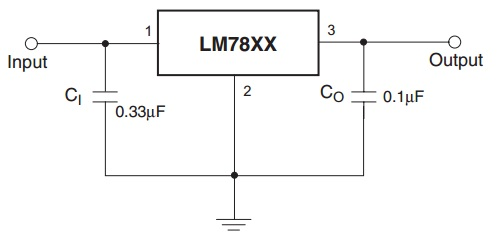
\includegraphics[width=0.7\linewidth]{Rysunki/78xx.jpg}
\caption{Schemat podłączenia układu zasilania \cite{LM78XX}}
\label{fig:LM78XX}
\end{figure}

\subsubsection{Montaż}
\par Mikrokontroler został zamontowany w schowku przed fotelem pasażera (rys.~\ref{fig:arduino_schowek}).

\begin{figure}[!htb]
\centering
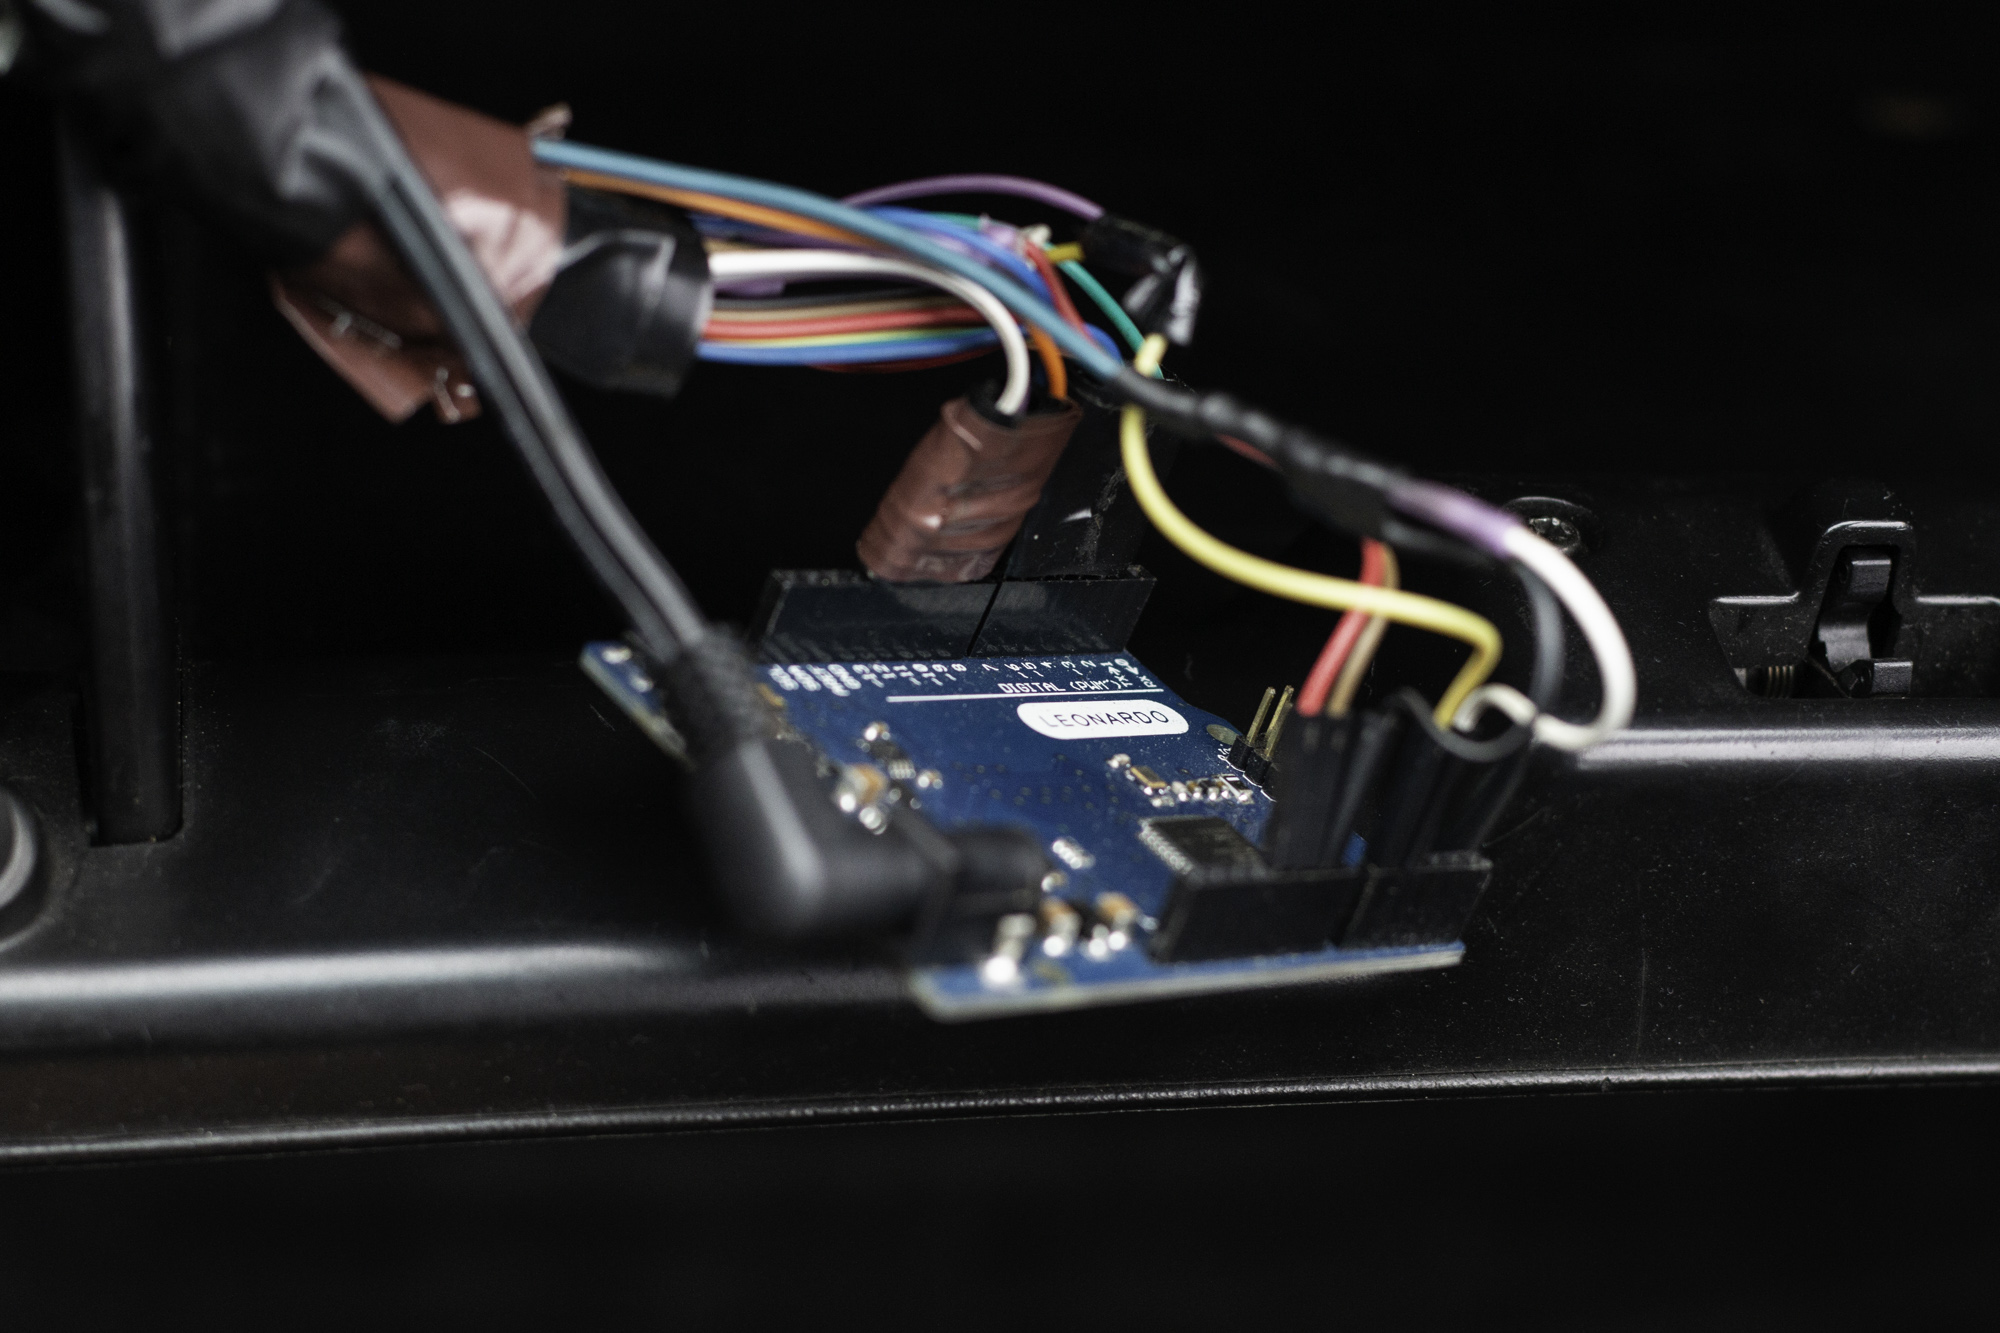
\includegraphics[width=0.8\linewidth]{Rysunki/arduino_schowek.jpg}
\caption{Mikrokontroler w schowku}
\label{fig:arduino_schowek}
\end{figure}

\section{Podłączenie do pojazdu}
\subsubsection{Komputer pokładowy}
Dostęp do wymaganych parametrów potrzebnych do poprawnego działania projektu może zostać uzyskany dzięki znajomości schematu podłączeń komputera pokładowego (ECU) umieszczonego w samochodzie. Ze schematu portów wejścia/wyjścia\cite{HondaPinout} można wywnioskować, iż wszystkie potrzebne sygnały są wpięte do ECU. Sygnały te zostały opisane w tabeli~\ref{tab:ecu_pinout}

\begin{table}[htb] \small
\centering
\caption{Potrzebne wyprowadzenia według schematu ECU\cite{HondaPinout}}
\label{tab:ecu_pinout}
\begin{tabularx}{\linewidth}{|c|p{7cm}|c|c|X|} \hline\
\textbf{Oznaczenie} & \textbf{Opis} & \textbf{Wtyczka} &\textbf{ Pin} & \textbf{Kolor} \\ 
\hline
INJ1 & Przewód do wtrysku pierwszego & A & 1 & brązowy\\
\hline
VSS & Przewód czujnika prędkości & B & 10 & żółty\\
\hline
TPS & Przewód czujnika położenia pedału gazu & D & 11 & jasny zielony\\
\hline
\end{tabularx}
\end{table}

Do podpięcia się do wyżej wymienionych przewodów zostały użyte bezinwazyjne szybkozłączki. 

\subsubsection{Czujnik prędkości} \label{vss}
Po wykonaniu pomiarów multimetrem okazało się, że impulsy w VSS mają dokładnie 5V, co oznacza, że nie potrzeba zastosowywać żadnych elementów elektronicznych, aby podłączyć się do modułu. Połączenie zostało więc stworzone bezpośrednio do pinu 7 obsługującego przerwanie 4.

\subsubsection{Sygnał wtrysku} \label{inj}
Wyniki pomiarów wykazały, iż wtryski pracują na napięciu 12V. W przypadku, gdy wtrysk nie wstrzykuje paliwa sygnał ma napięcie 12V, gdy pracuje jest to wartość poniżej 3V. W tej sytuacji trzeba zastosować element zmniejszający napięcie. W tym celu został wybrany stabilizator 7805. Dodatkowe kondensatory nie zostały użyte jak w przypadku układu zasilania Arduino, ponieważ mogłyby one wpływać na dokładność pomiarów. Przewód ze zmniejszonym już napięciem został podpięty do pinu 2 obsługującego przerwanie 1.

\subsubsection{Czujnik położenia pedału gazu}
Wyniki pomiarów wykazały, że czujnik ten działa niczym potencjometr i zmienia napięcie od \textasciitilde0.5V dla pedału nie wciśniętego wcale, do \textasciitilde4.5V gdy pedał jest wciśnięty w 100\%. Wyprowadzenie te zostało podłączone do analogowego pinu A0.

\subsubsection{Podłączenie woltomierza} \label{voltometer}

Ważną kwestią w przypadku woltomierza jest fakt, iż napięcie w układzie samochodu jest znacznie wyższe niż napięcie, na którym pracuje moduł. Nie zmniejszenie napięcia mogłoby skutkować uszkodzeniem modułu. Rozwiązaniem na ten problem jest zastosowanie układu z dwoma rezystorami (rys.~\ref{fig:voltometer}). Ten prosty obwód pozwolił na odpowiednie skalowanie wartości napięcia, aby nie przekraczało ono 5V. 
W ten sposób można modułem 5V mierzyć napięcie w zakresie 0-20V. Więcej informacji w podrozdziale \ref{voltometer_code}.

\begin{figure}[!htb]
\centering
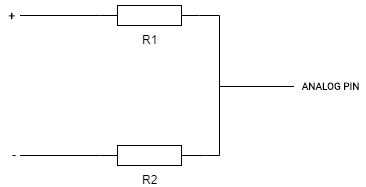
\includegraphics[width=0.7\linewidth]{Rysunki/voltometer_schemat.png}
\caption{Schemat podłączenia układu woltomierza}
\label{fig:voltometer}
\end{figure}


\section{Podłączenie akcesoriów}

\subsubsection{Mikro przełącznik}
Mikroprzełącznik, który tworzy integralną część modułu - dzięki niemu użytkownik może sterować trybami pracy modułu, został podłączony do pinu 13.

\subsubsection{Czujnik temperatury}
Dodatkową funkcją modułu będzie wyświetlanie aktualnej zewnętrznej temperatury. W tym celu został użyty cyfrowy czujnik temperatury DS18B20\cite{DS18B20_datasheet} w wersji wodoodpornej, 3 metrowej sondy. Czujnik ten umożliwia komunikację po interfejsie 1-Wire, dzięki któremu wystarczy tylko jedna linia, aby komunikować się z czujnikiem (więcej informacji w podrozdziale \ref{one_wire_temp}). W celu skorzystania z interfejsu 1-Wire potrzebny jest rezystor 4,7 k\textOmega, aby podciągnąć go do zasilania.

\subsubsection{Wyświetlacz LCD}
Wyświetlacz jaki został wybrany do projektu to znany model LCD z 2x16 znakami o symbolu JHD162A-B-W zgodny ze sterownikiem HD44780 \cite{HD44780_datasheet}. Został on połączony z Arduino poprzez cyfrowe piny: 12, 11, 6, 5, 4, 3. Dodatkowo został dołączony potencjometr do regulacji kontrastu wyświetlacza oraz zostało użyte dodatkowe połączenie służące do sterowania podświetleniem wyświetlacza - pin 9.

\par Wyświetlacz wraz z mikro przełącznikiem został osadzony przy kierownicy (rys.~\ref{fig:arduino_lcd}).
\begin{figure}[!h]
\centering
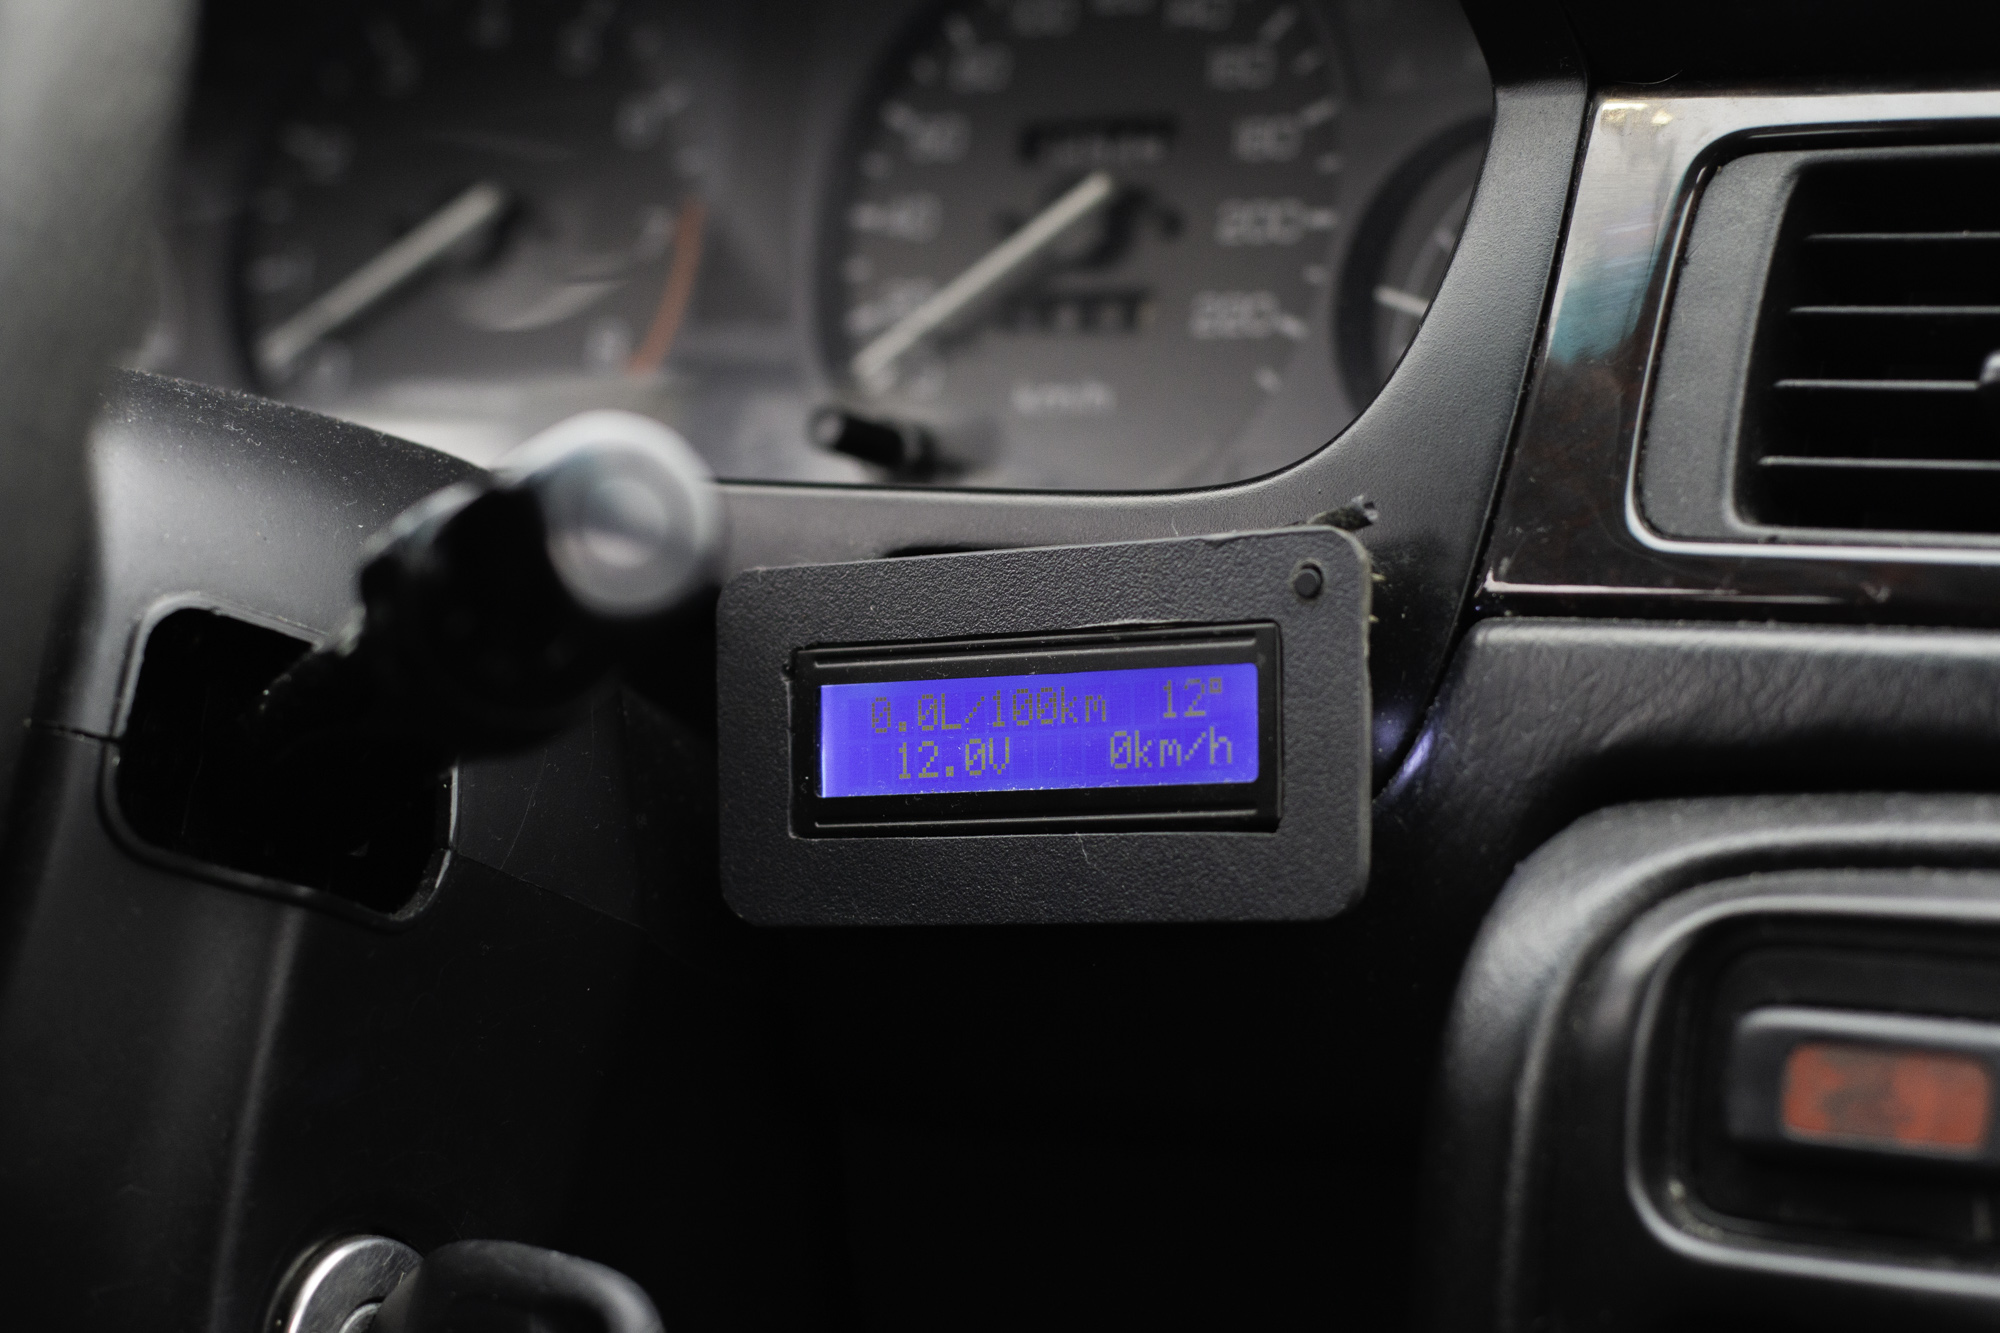
\includegraphics[width=0.8\linewidth]{Rysunki/arduino_lcd.jpg}
\caption{Miejsce osadzenia wyświetlacza}
\label{fig:arduino_lcd}
\end{figure}

\chapter{Programowanie i konfiguracja modułu}
\section{Środowisko programistyczne}
\chapter{Interfejs}
\section{Wprowadzenie}
W poprzednich rozdziałach został pokazany proces podłączania kolejnych modułów, konfiguracji ich oraz przetwarzania danych, w tym rozdziale ukazany zostanie interfejs, który już bezpośrednio będzie obsługiwany przez użytkownika końcowego.\\

Główny interfejs został podzielony na 3 karty menu, które są wybieralne przełącznikiem. Dodatkowo, w przypadku, gdy pojazd zatrzymał się, karta zmienia się automatycznie na alternatywną czwartą kartę, która pokazuje statystyki z przejazdu. Kolejną funkcjonalnością jest przytrzymanie przełącznika, które w zależności od aktualnej karty albo resetuje zapisane dane w pamięci, albo wyłącza podświetlenie ekranu.
\section{Implementacja}

\subsection{Odświeżanie}
\subsubsection{Wyświetlacz}
W przypadku, gdy odświeżanie wykonywałoby się bardzo szybko ekran LCD zacząłby migotać co utrudniałoby odczyt danych. Z tego powodu odświeżanie informacji na ekranie odbywa się co jedną sekundę. Zostało to zaimplementowane przy użyciu funkcji \texttt{millis()}, która zwraca liczbę milisekund od włączenia programu, podzielonej modulo 1000 (1 sekunda). W ten sposób, gdy wartość tego zapytania wynosi 0 przesyłane są nowe informacje do LCD.

\begin{lstlisting}[label=list:refresh_rate,caption=Implementacja odświeżania ekranu,
basicstyle=\footnotesize\ttfamily]
const czas_odswiezania_lcd = 1000;
---
void loop()
{
    ---
    if (millis() % czas_odswiezania_lcd == 0) 
    {
        // instrukcje dla wyświetlacza
    }
    ---
}

\end{lstlisting}

\subsubsection{Temperatura}
Jako, iż temperatura nie zmienia się tak szybko, a jej odczyt trwa chwilę czasu zostało postanowione, że będzie ona pobierana co 60 sekund oraz 2,5 sekundy po starcie programu.
\begin{lstlisting}[label=list:temp_refresh_rate,caption=Implementacja odświeżania temperatury,
basicstyle=\footnotesize\ttfamily]
const czas_odswiezania_temperatury = 60000;
float temp = 0.0;
---
void loop()
{
    ---
    if (millis() % czas_odswiezania_temperatury == 0 || millis() == 2500)
    {
        temp = temperatura();
    }
    ---
}

\end{lstlisting}

\subsection{Wyświetlanie i formatowanie danych}
\subsubsection{Prędkość}
Do wyświetlania aktualnej prędkości w formacie \textit{XXXkm/h} została przygotowana funkcja \texttt{wyswietlaniePredkosci(int X, int Y)}, która przyjmuje parametry X i Y, które oznaczają współrzędne wyświetlenia prędkości na wyświetlaczu.
\begin{lstlisting}[label=list:show_speed,caption=Wyświetlanie prędkości,
basicstyle=\footnotesize\ttfamily]
void wyswietlaniePredkosci(int X, int Y)
{
    lcd.setCursor(X, Y);
    lcd.print(predkosc, 0);
    lcd.print("km/h");
    lcd.setCursor(X - 3, Y);
    lcd.print("   ");
    if (predkosc >= 0 && predkosc < 10)
    	lcd.setCursor(X - 1, Y);
    else if (predkosc >= 10 && predkosc < 100)
    	lcd.setCursor(X - 2, Y);
    else if (predkosc >= 100)
    	lcd.setCursor(X - 3, Y);
}
\end{lstlisting}
\subsubsection{Spalanie na 100km}
Do wyświetlania aktualnego spalania w formacie \textit{XX.XL/100km} została przygotowana funkcja \texttt{wyswietlanieSpalaniaNa100(int X, int Y)}, która przyjmuje parametry X i Y, które oznaczają współrzędne wyświetlenia spalania na wyświetlaczu.
\begin{lstlisting}[label=list:show_fuel_cons_100,caption=Wyświetlanie spalania na 100km,
basicstyle=\footnotesize\ttfamily]
void wyswietlanieSpalaniaNa100(int X, int Y)
{
    lcd.setCursor(X + 4, Y);
    lcd.print("L/100km");
    lcd.setCursor(X + 1, Y);
    if (predkosc < 5)
    	lcd.print("0.0");
    else
    {
    	if (spalanieSto < 10)
    		lcd.print(spalanieSto, 1);
    	else if (spalanieSto >= 10)
    	{
    		lcd.setCursor(X, Y);
    		lcd.print(spalanieSto, 1);
    	}
    }
}
\end{lstlisting}

\subsubsection{Spalanie na godzinę}
Do wyświetlania aktualnego spalania w formacie \textit{X.XL/h} została przygotowana funkcja \texttt{wyswietlanieSpalaniaNaGodzine(int X, int Y)}, która przyjmuje parametry X i Y, które oznaczają współrzędne wyświetlenia spalania na wyświetlaczu.
\begin{lstlisting}[label=list:show_fuel_cons_hour,caption=Wyświetlanie spalania na godzinę,
basicstyle=\footnotesize\ttfamily]
void wyswietlanieSpalaniaNaGodzine(int X, int Y)
{
    lcd.setCursor (X + 3, Y);
	lcd.print("L/h");
	lcd.setCursor (X, Y);
	lcd.print(spalanieH, 1);
}
\end{lstlisting}

\subsubsection{Temperatura}
Do wyświetlania temperatury w formacie \textit{XX°} została przygotowana funkcja \texttt{wyswietlanieTemperatury(int X, int Y)}, która przyjmuje parametry X i Y, które oznaczają współrzędne wyświetlenia temperatury na wyświetlaczu.
\begin{lstlisting}[label=list:show_tempr,caption=Wyświetlanie temperatury,
basicstyle=\footnotesize\ttfamily]
void wyswietlanieTemperatury(int X, int Y)
{
    lcd.setCursor(X + 3, Y);
    lcd.print((char)223);
    lcd.setCursor(X, Y);
    lcd.print("   ");
    if (temp < 10 && temp >= 0)
    	lcd.setCursor(X + 2, Y);
    else if (temp >= 10 || (temp < 0 && temp >= -10) )
    	lcd.setCursor(X + 1, Y);
    else if (temp <= 10)
    	lcd.setCursor(X, Y);
    lcd.print(temp, 0);
}
\end{lstlisting}

\subsubsection{Napięcie}
Do wyświetlania aktualnego napięcia w formacie \textit{XX.XV} została przygotowana funkcja \texttt{wyswietlanieNapiecia(int X, int Y)}, która przyjmuje parametry X i Y, które oznaczają współrzędne wyświetlenia napięcia na wyświetlaczu.
\begin{lstlisting}[label=list:show_voltage,caption=Wyświetlanie napięcia,
basicstyle=\footnotesize\ttfamily]
void wyswietlanieNapiecia(int X, int Y)
{
    lcd.setCursor(X, Y);
    lcd.print(woltomierz(),1);
    lcd.setCursor(X + 4, Y);
    lcd.print("V");
}
\end{lstlisting}

\subsubsection{Przejechany dystans}
Do wyświetlania przejechanego dystansu w formacie \textit{XXXkm} została przygotowana funkcja \texttt{wyswietlanieDystansu(int X, int Y)}, która przyjmuje parametry X i Y, które oznaczają współrzędne wyświetlenia dystansu na wyświetlaczu.
\begin{lstlisting}[label=list:show_millage,caption=Wyświetlanie dystansu,
basicstyle=\footnotesize\ttfamily]
void wyswietlanieDystansu(int X, int Y)
{
    lcd.setCursor(X, Y);
    lcd.print(trip);
    lcd.print("km");
}
\end{lstlisting}

\subsubsection{Spalone paliwo}
Do wyświetlania spalonego paliwa w formacie \textit{XX.XL} została przygotowana funkcja \texttt{wyswietlanieSpalonegoPaliwa(int X, int Y)}, która przyjmuje parametry X i Y, które oznaczają współrzędne wyświetlenia spalonego paliwa na wyświetlaczu.
\begin{lstlisting}[label=list:show_fuel_burned,caption=Wyświetlanie spalonego paliwa,
basicstyle=\footnotesize\ttfamily]
void wyswietlanieSpalonegoPaliwa(int X, int Y)
{
    lcd.setCursor(X, Y);
    lcd.print(spalone, 2);
    if(spalone < 10)
    	lcd.setCursor (X + 4, Y);
    else
    	lcd.setCursor (X + 4, Y);
    lcd.print("L");
}
\end{lstlisting}

\subsubsection{Średnie spalanie na 100 km}
Do wyświetlania średniego spalonego paliwa na 100 km w formacie \textit{•XX.X} została przygotowana funkcja \texttt{wyswietlanieSredniegoSpalania(int X, int Y)}, która przyjmuje parametry X i Y, które oznaczają współrzędne wyświetlenia średniego spalonego paliwa na wyświetlaczu.
\begin{lstlisting}[label=list:show_fuel_avarge,caption=Wyświetlanie średniego spalonego paliwa na 100km,
basicstyle=\footnotesize\ttfamily]
void wyswietlanieSredniegoSpalania(int X, int Y)
{
    lcd.setCursor (X, Y);
    lcd.print((char)243);
    lcd.setCursor (X + 1, 1);
    if (trip == 0.0)
    	lcd.print("0.0");
    else
    	lcd.print((100/trip)*spalone, 1);
}
\end{lstlisting}

\subsubsection{Położenie pedału gazu}
Kontroler sterujący wyświetlaczem umożliwia manualne stworzenie znaków. Dzięki tej opcji zostały stworzone specjalne znaki, które graficznie pokazują nacisk pedału. Działają one na zasadzie paska postępu, który ładuje się z dołu do góry w zależności od wciśnięcia pedału gazu.

\begin{lstlisting}[label=list:custom_char,caption=Tworzenie znaków specjalnych dla odczytu pedału gazu,
basicstyle=\footnotesize\ttfamily]
byte a1[8] = {B00000,B00000,B00000,B00000,B00000,B00000,B00000,B11111};
byte a2[8] = {B00000,B00000,B00000,B00000,B00000,B00000,B11111,B11111};
byte a3[8] = {B00000,B00000,B00000,B00000,B00000,B11111,B11111,B11111};
byte a4[8] = {B00000,B00000,B00000,B00000,B11111,B11111,B11111,B11111};
byte a5[8] = {B00000,B00000,B00000,B11111,B11111,B11111,B11111,B11111};
byte a6[8] = {B00000,B00000,B11111,B11111,B11111,B11111,B11111,B11111};
byte a7[8] = {B00000,B11111,B11111,B11111,B11111,B11111,B11111,B11111};
byte a8[8] = {B11111,B11111,B11111,B11111,B11111,B11111,B11111,B11111};
---
void setup()
{
    ---
    lcd.createChar(0, a1);
	lcd.createChar(1, a2);
	lcd.createChar(2, a3);
	lcd.createChar(3, a4);
	lcd.createChar(4, a5);
	lcd.createChar(5, a6);
	lcd.createChar(6, a7);
	lcd.createChar(7, a8);
    ---
}
\end{lstlisting}

Do wyświetlania aktualnego położenia pedału gazu została przygotowana funkcja \texttt{wyswietlaniePolozeniaPedaluGazu(int X, int Y)}, która przyjmuje parametry X i Y, które oznaczają współrzędne wyświetlenia odczytu na wyświetlaczu.
\begin{lstlisting}[label=list:show_fuel_avarge,caption=Wyświetlanie średniego spalonego paliwa na 100km,
basicstyle=\footnotesize\ttfamily]
float nacisk = 0.0;
void wyswietlaniePolozeniaPedaluGazu(int X, int Y)
{
    nacisk = aktualnyNacisk();
    lcd.setCursor (X, Y);
    if (nacisk <= 3)
    	lcd.print(" ");
    else if (nacisk > 3 && nacisk <= 12.5)
    	lcd.write(byte(0));
    else if (nacisk > 12.5 && nacisk <= 25)
    	lcd.write(byte(1));
    else if (nacisk > 25 && nacisk <= 37.5)
    	lcd.write(byte(2));
    else if (nacisk > 37.5 && nacisk <= 50)
    	lcd.write(byte(3));
    else if (nacisk > 50 && nacisk <= 62.5)
    	lcd.write(byte(4));
    else if (nacisk > 62.5 && nacisk <= 75)
    	lcd.write(byte(5));
    else if (nacisk > 75 && nacisk <= 87.5)
    	lcd.write(byte(6));
    else if (nacisk > 87.5)
    	lcd.write(byte(7));
    }
}
\end{lstlisting}

\subsection{Menu i karty}
Obsłużenie kart menu polega na inkrementacji zmiennej \texttt{menu} podczas naciskania przycisku. W zależności wartości tej zmiennej wyświetlana jest inna karta menu.

\subsubsection{Obsługa menu}

\begin{lstlisting}[label=list:menu,caption=Implementacja obsługi menu,
basicstyle=\footnotesize\ttfamily]
int menu = 1;

void nacisnieciePrzycisku()
{
    if (menu > 3)
        menu = 1;
    else
        menu++;
}
---
void loop()
{
    ---
    switch (menu) 
    {
        case 1:
            menu1();
            break;
        case 2:
            menu2();
            break;
        case 3:
            menu2();
            break;
    }
    ---
}
\end{lstlisting}

\subsubsection{Pierwsza karta}

Zostało założone, że pierwsza karta będzie tą najczęściej używaną, więc znalazły się na niej najczęściej potrzebne parametry: prędkość, spalanie na 100km, temperatura, napięcie w układzie i położenie pedału gazu. Podgląd tej można zobaczyć na rysunku (rys.~\ref{fig:menu1}).

\begin{figure}[!htb]
\centering
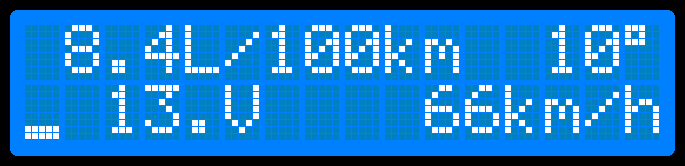
\includegraphics[width=0.7\linewidth]{Rysunki/menu1.png}
\caption{Podgląd pierwszej karty menu}
\label{fig:menu1}
\end{figure}

\subsubsection{Druga karta}
Na drugiej karcie znalazły się informacje na temat przejechanego dystansu oraz spalonego paliwa. Podgląd tej można zobaczyć na rysunku (rys.~\ref{fig:menu2}).

\begin{figure}[!htb]
\centering
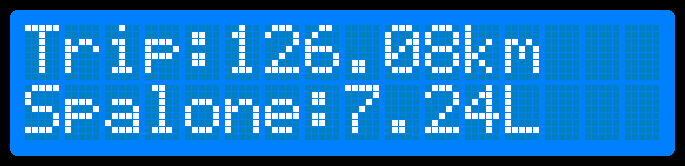
\includegraphics[width=0.7\linewidth]{Rysunki/menu2.png}
\caption{Podgląd drugiej karty menu}
\label{fig:menu2}
\end{figure}

\subsubsection{Trzecia karta}
Na trzeciej karcie znajdują się informacje na temat spalania: spalanie na 100 km, spalanie na godzinę oraz średnie spalanie na 100 km.Podgląd tej można zobaczyć na rysunku (rys.~\ref{fig:menu3}).

\begin{figure}[!htb]
\centering
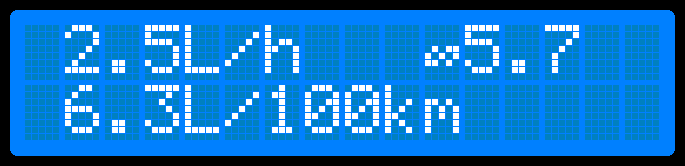
\includegraphics[width=0.7\linewidth]{Rysunki/menu3.png}
\caption{Podgląd trzeciej karty menu}
\label{fig:menu3}
\end{figure}


\subsubsection{Karta przy postoju}
Na tej karcie znalazły się informacje na temat średniego spalania, spalonego paliwa, aktualnego spalania na godzinę oraz przejechanego dystansu. Podgląd tej można zobaczyć na rysunku (rys.~\ref{fig:menu0}).

\begin{figure}[!htb]
\centering
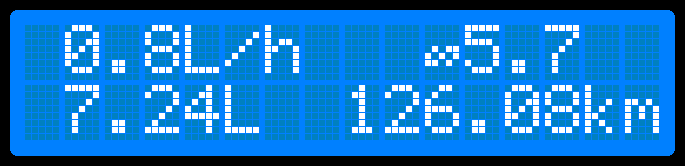
\includegraphics[width=0.7\linewidth]{Rysunki/menu0.png}
\caption{Podgląd postojowej karty menu}
\label{fig:menu0}
\end{figure}

Karta ta wyświetlana jest tylko wtedy, gdy prędkość pojazdu spadnie poniżej 2 km/h oraz przejechany dystans jest większy niż 200 m.
\begin{lstlisting}[label=list:menu_card4,caption=Włączanie karty podczas postoju,
basicstyle=\footnotesize\ttfamily]
---
void loop()
{
    ---
    if (predkosc < 2.0 && trip > 0.2)
    {
        menu0();
    }
    ---
}
\end{lstlisting}



\subsection{Resetowanie zapisanych danych}
Aby umożliwić użytkownikowi zerowanie zapisanych danych została stworzona funkcja \texttt{resetuj()}. Można ją wywołać przytrzymując przycisk jednocześnie będąc na 2 karcie menu.

\begin{lstlisting}[label=list:menu_card4,caption=Resetowanie zapisanych danych,
basicstyle=\footnotesize\ttfamily]
---
void resetuj()
{
    EEPROMWritelong(0, 0);
    EEPROMWritelong(4, 0);
    dystans = 0;
    trip = 0;
}
void przytrzymaniePrzycisku()
{
    switch (menu)
    {
    ---
    case 2:
        resetuj();
        break;
    ---
    }
}
---
\end{lstlisting}

\subsection{Sterowanie podświetleniem}
Moduł umożliwia również sterowanie podświetleniem poprzez zmianę stanu portu. Zostały stworzone dwa tryby podświetlenia: domyślny (pełna jasność) oraz wyłączony (nocny). Można je przełączać przytrzymaniem przycisku, gdy aktualną kartą menu jest karta pierwsza.

\begin{lstlisting}[label=list:hold_button_brightness,caption=Resetowanie zapisanych danych,
basicstyle=\footnotesize\ttfamily]
bool jasnosc = true;
const jasnosc_pin = 9;
---
void setup()
{
    ---
    digitalWrite(jasnosc_pin, jasnosc);
    ---
}
void przelaczPodswietlenie()
{
    jasnosc = !jasnosc;
    digitalWrite(jasnoscPin, jasnosc);
}
void przytrzymaniePrzycisku()
{
    switch (menu)
    {
    ---
    case 1:
        przelaczPodswietlenie();
        break;
    ---
    }
}
---
\end{lstlisting}
\chapter{Podsumowanie}
\section{Zdjęcia implementacji}
\section{Wykonane prace}
\section{Możliwości rozbudowy}

%\bibliographystyle{plalpha}
\bibliographystyle{unsrt}

%UWAGA: bibliotekę referencji należy przygotować samemu. Dobrym do tego narzędziem jest JabRef.
%       Nazwę przygotowanej biblioteki wpisuje się poniżej bez rozszerzenia 
%       (w tym przypadku jest to "dokumentacja.bib")
\bibliography{dokumentacja}
\appendix

\chapterstyle{noNumbered}
\phantomsection % sets an anchor
\printindex

\end{document}
